\chapter[Desarrollo de firmware]{Desarrollo de firmware}
\label{cp:desarrolloFirmware}

\section{Interfaz de Comunicación}

La interfaz de comunicación constituye la capa de abstracción encargada de desacoplar los medios de comunicación físicos y lógicos del resto del sistema. Su propósito es proporcionar una API uniforme que permita a las capas superiores operar independientemente del mecanismo de transporte utilizado.

Esta capa define un contrato común de interacción entre las distintas implementaciones de comunicación (puerto serie, USBTMC, GPIB, VXI-11, HiSLIP, entre otras) y el subsistema encargado del procesamiento de comandos y respuestas. Cada implementación adapta dicho contrato a las características particulares del medio de comunicación subyacente, permitiendo que las capas superiores permanezcan independientes de los detalles específicos de cada tecnología.

El diseño persigue los siguientes objetivos:

\begin{itemize}
\item Independencia del hardware y del medio de comunicación subyacente.
\item Reutilización del subsistema de comunicación sobre múltiples tecnologías de transporte.
\item Uniformidad en el acceso a los servicios de transmisión y recepción de datos.
\item Manejo uniforme de estados, eventos y errores.
\item Escalabilidad para incorporar nuevas interfaces de comunicación sin modificar las capas superiores.
\item Compatibilidad con protocolos de instrumentación basados en texto, particularmente SCPI.
\end{itemize}

La interfaz de comunicación no implementa funcionalidades de protocolo de aplicación ni procesamiento de comandos. Su responsabilidad consiste en administrar el acceso al medio de comunicación, coordinar la transferencia de datos y exponer de manera uniforme los estados, eventos y errores relevantes para las capas superiores.

Desde el punto de vista arquitectónico, la interfaz de comunicación representa el límite entre la capa dependiente de la implementación de transporte y la capa independiente de la tecnología utilizada.

\subsection{Conceptos Fundamentales}

Con el fin de establecer una terminología común para el resto de la arquitectura, la interfaz de comunicación se apoya en los siguientes conceptos fundamentales.

\paragraph{Estado}

Un estado representa una condición persistente de una interfaz de comunicación durante un intervalo de tiempo.

Los estados describen la situación operativa actual de una interfaz, por ejemplo, si se encuentra disponible, conectada, transmitiendo datos o procesando una recepción.

A diferencia de los eventos, los estados permanecen vigentes hasta que una nueva condición los modifica.

\paragraph{Evento}

Un evento representa la ocurrencia instantánea de una situación relevante para el sistema.

Ejemplos típicos de eventos son la disponibilidad de nuevos datos, la finalización de una transmisión o la detección de una condición de error.

Los eventos no representan condiciones permanentes sino notificaciones puntuales que deben ser procesadas por las capas superiores.

\paragraph{Error}

Un error representa una condición anómala detectada durante la operación de la interfaz.

Los errores pueden originarse tanto en el medio de comunicación subyacente como en mecanismos internos de la propia implementación.

La detección de un error no implica necesariamente la interrupción del servicio, pero sí requiere que la condición sea informada mediante los mecanismos definidos por la interfaz.

\paragraph{Operación}

Una operación representa una acción solicitada por una capa superior sobre una interfaz de comunicación.

Las operaciones constituyen el conjunto de servicios ofrecidos por la interfaz y permiten controlar su comportamiento sin exponer detalles específicos de implementación.

Ejemplos de operaciones son la inicialización de una interfaz, el inicio de una transmisión o el reinicio de una instancia de comunicación.

\paragraph{Contexto}

El contexto es una estructura de datos privada asociada a una instancia concreta de interfaz.

Su contenido depende de la implementación particular y almacena toda la información necesaria para administrar el medio de comunicación correspondiente.

Las capas superiores no acceden directamente al contexto ni dependen de su estructura interna.

\paragraph{Propietario}

El propietario de un recurso es el componente responsable de administrar su ciclo de vida y garantizar su validez.

La interfaz define explícitamente la propiedad de los recursos compartidos para evitar dependencias implícitas entre módulos.

Esta definición resulta especialmente importante para las estructuras utilizadas durante la transferencia de datos, permitiendo establecer responsabilidades claras respecto de su creación, utilización y liberación.

\subsection{Responsabilidades de la Interfaz}

La interfaz de comunicación es responsable de:

\begin{itemize}
\item Inicializar y configurar la implementación de comunicación asociada.
\item Configurar y administrar los recursos necesarios para la transferencia de datos.
\item Gestionar la recepción de información proveniente del medio de comunicación.
\item Iniciar transmisiones solicitadas por las capas superiores.
\item Detectar eventos relevantes producidos por la implementación subyacente.
\item Detectar y reportar errores de comunicación.
\item Publicar eventos hacia el subsistema de comunicación.
\item Mantener el estado operativo interno de la interfaz.
\end{itemize}

\subsection{Responsabilidades Excluidas}

Las siguientes funciones quedan explícitamente fuera del alcance de esta capa:

\begin{itemize}
\item Procesamiento de comandos SCPI.
\item Interpretación de protocolos de aplicación.
\item Validación sintáctica de mensajes.
\item Gestión de sesiones.
\item Generación de respuestas.
\item Almacenamiento persistente de configuraciones.
\item Coordinación de tareas de aplicación.
\end{itemize}

La exclusión de estas responsabilidades permite mantener una separación estricta entre los mecanismos de transporte y la lógica funcional del instrumento.

\subsection{Modelo de Interacción}

La comunicación entre la interfaz y las capas superiores se basa en un modelo orientado a eventos. Si tomamos los eventos de interfaz de recepcion y los datos de entrada como entradas del sistema, el sistema de recepcion sera una maquina de Mealy que funcinara con sus estados internos y las entradas mencionadas. 
En este contexto los evetos puede ser mucho mejor implementarlos como un bitmask

Las capas superiores consumen dichos eventos y toman las acciones correspondientes.

Este enfoque evita dependencias directas entre las implementaciones de comunicación y las tareas de aplicación, favoreciendo una arquitectura desacoplada.

Conceptualmente, la interacción sigue el siguiente flujo:

\begin{center}
Medio de Comunicación $\rightarrow$ Interfaz de Comunicación $\rightarrow$ Eventos $\rightarrow$ Subsistema de Comunicación $\rightarrow$ Motor SCPI
\end{center}

La transmisión de datos sigue el camino inverso:

\begin{center}
Motor SCPI $\rightarrow$ Subsistema de Comunicación $\rightarrow$ Interfaz de Comunicación $\rightarrow$ Medio de Comunicación
\end{center}

Un esquema simplificado del sisema se puede ver el la figura \ref{fig:esquema-comunicacion}.

\begin{figure}[htbp]
    \centering
    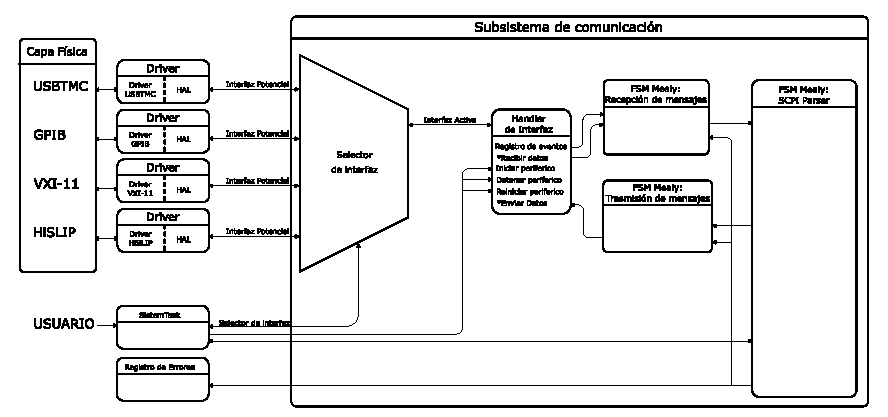
\includegraphics[width=1.0\linewidth]{Figuras/Schems/subsitema-comunicacion_mealy.pdf}
    \caption{Sistema de comunicación.}
    \label{fig:esquema-comunicacion}
\end{figure}

\subsection{Elección del Medio de Transporte}

El subsistema de comunicación opera exclusivamente sobre la interfaz abstracta definida por esta capa y no depende de ninguna implementación particular.

La asociación entre el subsistema de comunicación y una implementación concreta es realizada por un selector de interfaz. Este componente determina cuál de las interfaces disponibles será utilizada por el sistema de acuerdo con la configuración activa del instrumento.

El selector de interfaz no participa en la transferencia ni en el procesamiento de datos. Su única responsabilidad consiste en establecer la asociación entre el subsistema de comunicación y una interfaz de comunicación determinada.

Como consecuencia, el medio de transporte puede modificarse sin requerir cambios en las capas superiores del sistema. Un mismo subsistema de comunicación puede operar sobre USBTMC, GPIB, VXI-11, HiSLIP u otras interfaces compatibles manteniendo inalterada la lógica de procesamiento de comandos y respuestas.

